\documentclass[fontset=windows,16pt]{ctexart}  
\usepackage{graphicx}
\usepackage{amsmath}
\usepackage{booktabs}
\usepackage{float}
\usepackage{titlesec}
\usepackage{ulem}  
\usepackage[left=3cm,right=3cm,top=3cm,bottom=3cm]{geometry}  
\usepackage{fancyhdr}  % 用于定制页眉页脚

% 页眉页脚设置
\pagestyle{fancy}
\fancyhf{}  % 清空默认页眉页脚
\fancyhead[C]{\zihao{5}\bfseries 仿真实验报告(一)}  % 居中页眉:报告标题
\fancyhead[R]{\zihao{5} 小美\ \ \ 三年级一班}  % 右侧页眉:姓名+班级
\fancyfoot[C]{\thepage}  % 居中页脚:页码
\renewcommand{\headrulewidth}{0.5pt}  % 页眉下划线宽度
\renewcommand{\footrulewidth}{0pt}  % 取消页脚下划线

% 自定义一级标题格式为中文编号"一、二、",居左显示
\titleformat{\section}
  {\normalfont\Large\bfseries\fontsize{18pt}{22pt}\selectfont}
  {\chinese{section}、}{0.5em}{}
\titlespacing*{\section}{0pt}{1.5ex plus 0.5ex minus 0.5ex}{1ex plus 0.2ex minus 0.2ex}

% 二级标题保持阿拉伯数字编号格式不变
\titleformat{\subsection}
  {\normalfont\bfseries\fontsize{16pt}{20pt}\selectfont}
  {\thesubsection、}{0.5em}{}
\titlespacing*{\subsection}{0pt}{1ex plus 0.5ex minus 0.5ex}{0.5ex plus 0.2ex minus 0.2ex}

\title{%
  \vspace{-2em}  % 减小标题与顶部的间距
  \begin{center}
    
\includegraphics[width=0.4\textwidth]{img/logo.png}  % 插入校徽图片,替换为指定图片
    
    \vspace{1em}  % 图片与标题的间距
    
    \fontsize{26pt}{20pt}\selectfont
    \CJKsetecglue{\hskip 1em plus 0pt minus 0pt}
    物\ \ \ \ 理\ \ \ \ 实\ \ \ \ 验\ \ \ \ 报\ \ \ \ 告
  \end{center}
}
\date{}
\begin{document}


\maketitle

% 个人信息排版:用tabular居中,带单下划线
\vspace{-5.5ex} 
\begin{center}
\begin{tabular}{@{}c@{}c@{}c@{}c@{}}
班级\underline{\hspace{1em}三年级一班\hspace{1em}} & 姓名\underline{\hspace{1em}小美\hspace{1em}} & 学号\underline{\hspace{1em}10086\hspace{1em}} & 实验日期\underline{\hspace{1em}2025.6.12\hspace{1em}} \\
\end{tabular}
\vspace{0.3em}  % 个人信息与双下划线的间距
\uuline{\rule{\textwidth}{3pt}}  % 双下划线
\end{center}

% 实验名称排版:居中,下方加单下划线
\begin{center}
\vspace{0.5em} 
\zihao{3}\bfseries  % 三号字加粗
\fontsize{22pt}{22pt}\selectfont  % 设置字体大小
实验名称:密里根油滴实验\\
\vspace{-0.8em} 
\underline{\rule{0.6\linewidth}{0.1em}}  % 单下划线
\end{center}

\section{实验目的}
1. 了解密里根油滴仪的结构,掌握利用滴定法测定电子电荷的设计思路和方法。
\\
2. 了解CCD图像传感器的原理和电视显微测量方法
\\
3. 学会使用图示法处理数据


\section{实验原理}
根据油滴在电场中作直线运动或静止两种运动方式分类,油滴法测电子电荷分为动态测量法和平衡测量法。

\subsection{动态测量法}
考虑重力场中一个足够小油滴的运动,设此油滴半径为\( r \),质量为\( m_1 \),空气是粘滞流体,故此运动油滴除受重力和浮力作用外还受粘滞阻力的作用。由斯托克斯定律,粘滞阻力与物体运动速度成正比。设油滴以匀速\( v_f \)下落,则有
\[
m_1 g - m_2 g = K v_f \tag{1}
\]
此处\( m_2 \)为与油滴同体积空气的质量,\( K \)为比例常数,\( g \)为重力加速度。油滴在空气及重力场中的受力情况如图\ref{fig:force1}所示。

若此油滴带电荷为\( q \),并处在场强为\( E \)的均匀电场中,设电场力\( qE \)方向与重力方向相反,如图\ref{fig:force2}所示,如果油滴以匀速\( v_r \)上升,则有
\[
qE = (m_1 - m_2)g + K v_r \tag{2}
\]
由式(1)和(2)消去\( K \),可解出\( q \)为:
\[
q = \frac{(m_1 - m_2)g (v_f + v_r)}{E v_f} \tag{3}
\]

设油与空气的密度分别为\( \rho_1, \rho_2 \),于是半径为\( r \)的油滴的视重为:
\[
(m_1 - m_2)g = \frac{4}{3}\pi r^3 (\rho_1 - \rho_2)g \tag{4}
\]
由斯托克斯定律,粘滞流体对球形运动物体的阻力与物体速度成正比,其比例系数\( K \)为\( 6\pi\eta r \),此处\( \eta \)为粘度,\( r \)为物体半径,于是可将公式(4)带入式(1)有
\[
6\pi\eta r v_f = \frac{4}{3}\pi r^3 (\rho_1 - \rho_2)g \tag{5}
\]
因此,
\[
r = \sqrt{\frac{9\eta v_f}{2(\rho_1 - \rho_2)g}} \tag{6}
\]
以此带入(3)并整理得到
\[
q = \frac{18\pi\eta^{3/2} (\rho_1 - \rho_2)^{-1/2} g^{-1/2} (v_f + v_r) v_f^{1/2}}{E} \tag{7}
\]

考虑到油滴的直径与空气分子的间隙相当,空气已不能看成是连续介质,其粘度\( \eta \)需作相应的修正
\[
\eta' = \frac{\eta}{1 + \frac{b}{pr}}
\]
此处\( p \)为空气压强,\( b \)为修正常数,\( b = 0.00823\ \text{N/m} \),因此,
\[
r = \sqrt{\frac{9\eta v_f}{2(\rho_1 - \rho_2)g(1 + \frac{b}{pr})}} \tag{8}
\]
当精确度要求不太高时,常采用近似计算方法,先将\( v_f \)带入(6)式计算得
\[
r_0 = \sqrt{\frac{9\eta v_f}{2(\rho_1 - \rho_2)g}} \tag{9}
\]
再将此\( r_0 \)值带入\( \eta' \)中,并以\( \eta' \)入式(7),得
\[
q = \frac{18\pi\eta^{3/2} (\rho_1 - \rho_2)^{-1/2} g^{-1/2} (v_f + v_r) v_f^{1/2}}{E \left(1 + \frac{b}{pr_0}\right)^{3/2}} \tag{10}
\]

实验中常常固定油滴运动的距离,通过测量它通过此距离\( s \)所需的时间来求得其运动速度,且电场强度\( E = U/d \),\( d \)为平行板间的距离,\( U \)为所加的电压,因此,式(10)可写成
\[
q = \frac{18\pi\eta^{3/2} (\rho_1 - \rho_2)^{-1/2} g^{-1/2} d (t_f + t_r) t_f^{1/2}}{U s^{1/2} \left(1 + \frac{b}{pr_0}\right)^{3/2}} \tag{11}
\]
式中有些量和实验仪器以及条件有关,选定之后在实验过程中不变,如\( d \),\( s \),\( (\rho_1 - \rho_2) \)及\( \eta \)等,将这些量与常数一起用\( C \)代表,可称为仪器常数,于是式(11)简化成
\[
q = C \frac{(t_f + t_r) t_f^{1/2}}{U}
\]

\begin{figure}[H]
    \centering
    \begin{minipage}[t]{0.2\textwidth}
        \centering
        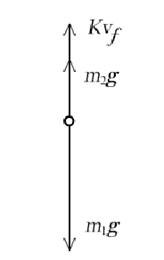
\includegraphics[width=\textwidth]{img/受力1.png.jpg}
        \caption{重力场中油滴受力示意图}
        \label{fig:force1}
    \end{minipage}
    \hspace{1cm} % 增加1厘米的间隔
    \begin{minipage}[t]{0.2\textwidth}
        \centering
        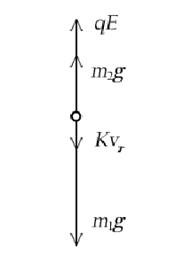
\includegraphics[width=\textwidth]{img/受力2.jpg}
        \caption{电场中油滴受力示意图}
        \label{fig:force2}
    \end{minipage}
\end{figure}

\subsection{平衡测量法}
平衡测量法的出发点是,使油滴在均匀电场中静止在某一位置,或在重力场中作匀速运动。

当油滴在电场中平衡时,油滴在两极板间受到的电场力\( qE \),重力\( m_1g \)和浮力\( m_2g \)达到平衡,从而静止在某一位置,即
\[
qE = (m_1 - m_2)g \tag{12}
\]
油滴在重力场中作匀速运动时,情形同动态测量法,将式(4),(9)和
\[
\eta' = \frac{\eta}{1 + \frac{b}{pr_0}}
\]
带入式(11)并注意到\( v_r = 0 \),则有
\[
q = \frac{18\pi\eta^{3/2} (\rho_1 - \rho_2)^{-1/2} g^{-1/2} d t_f^{1/2}}{U s^{1/2} \left(1 + \frac{b}{pr_0}\right)^{3/2}} \tag{13}
\]

\subsection{元电荷的测量方法}
测量油滴上带的电荷的目的是找出电荷的最小单位\( e \)。为此可以对不同的油滴,分别测出其所带的电荷值\( q_i \),它们应近似为某一最小单位的整数倍,即油滴电荷量的最大公约数,或油滴带电量之差的最大公约数,即为元电荷。

实验中采用紫外线,X射线或放射源等改变同一油滴所带的电荷,测量油滴上所带电荷的改变值\( \Delta q_i \),而\( \Delta q_i \)值应是元电荷的整数倍。
即
\[
\Delta q_i = n_j e \quad (\text{其中} \ n_j \ \text{为一整数}) \tag{14}
\]
也可以用作图法求\( e \)的值,根据式(14),\( e \)为直线方程的斜率,通过测量大量油滴的电量,拟合直线,即可求得\( e \)值。


\section{实验步骤及注意事项}

\subsection{选择适当的油滴并测量油滴上所带电荷}
要做好油滴实验,所选的油滴体积要适中,大的油滴虽然比较亮,但下降速度快,不容易测准确;太小则受布朗运动的影响明显,测量结果涨落很大,也不容易测准确。因此应该选择质量适中,而带电不多的油滴。

\subsection{调整油滴实验装置}
油滴实验装置由油滴盒、油滴照明装置、调平系统、测量显微镜、供电电源、电子停表及喷雾器等组成,其结构如图\ref{fig:apparatus}所示。其中油滴盒是由两块经过精磨的金属平板,中间垫以胶木圆环,构成的平行板电容器。在上板中心处有落油孔,使微小油滴可以进入电容器中间的电场空间,胶木圆环上有进光孔、观察孔。进入电场空间内的油滴由照明装置照明,油滴盒可通过调平螺旋调整水平,用水准仪检查。油滴盒防风罩前装有测量显微镜,用来观察油滴。

\begin{figure}[H]
    \centering
    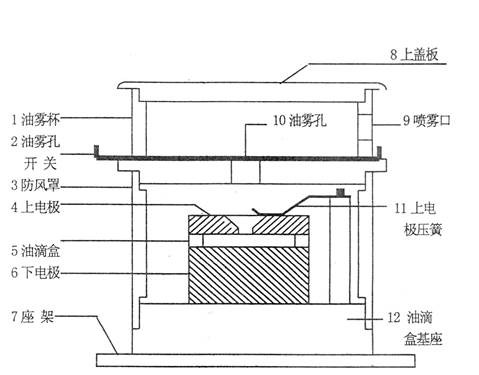
\includegraphics[width=0.7\textwidth]{img/装置.png.jpg}
    \caption{密里根油滴实验装置图}
    \label{fig:apparatus}
\end{figure}

电容器极板上所加电压由直流平衡电压和直流升降电压两部分组成。其中平衡电压大小连续可调,并可从显示屏上直接读数,其极性由换向开关控制,以满足对不同极性电压的需要。升降电压的大小可连续调节,并可通过换向开关叠加在平衡电压上,以控制油滴在电容器内上下的位置。

油滴实验是一个操作技巧要求较高的实验,为了得到满意的实验结果,必须仔细认真调整油滴仪,具体步骤如下:
\begin{enumerate}
\item 调节调平螺丝,将平行电极板调到水平,使平衡电场方向与重力方向平行,避免引起实验误差。
\item 调节显微镜焦点,使油滴清晰显示在显示屏上。
\item 喷雾器用于快速向油滴仪内喷油雾,喷射过程中由于摩擦作用可使油滴带电。
\end{enumerate}

当油雾从喷雾口喷入油滴室内后,视场中将出现大量清晰的油滴,此时可加上平衡电压,改变其大小和极性,驱散不需要的油滴,练习控制其中一颗油滴的运动,并记录油滴经过两条横丝间距所用的时间。

\subsection{正式测量}
\begin{enumerate}
\item 选取平衡电压约200V、匀速下降时间约20s—35s的油滴,测量油滴匀速运动2mm所用的时间。油滴过大则下降速度过快,过小则布朗运动明显,均会影响测量精度。

数据处理时所需的参数值如下:
\[
\begin{tabular}{|l|l|}
\hline
油密度 & $\rho = 981\ \text{kg} \cdot \text{m}^{-3}$ \\
\hline
空气密度 & $\rho = 1.29\ \text{kg} \cdot \text{m}^{-3}\ (20^\circ\text{C})$ \\
\hline
重力加速度 & 查当地值 \\
\hline
空气粘滞系数 & $\eta = 1.832 \times 10^{-5}\ \text{kg}/(\text{m} \cdot \text{s})\ (23^\circ\text{C})$ \\
\hline
平行板间距 & $d = 5 \times 10^{-3}\ \text{m}$ \\
\hline
修正系数 & $b = 8.23 \times 10^{-3}\ \text{N/m}$ \\
\hline
\end{tabular}
\]

\item 计算每个油滴的带电量,采用倒过来验证的方法:用公认的电子电量值去除每个油滴的电量,取最接近的整数,再用该整数除油滴的电量,得到电子电荷的测量值。

\item 将电子电荷的测量值与理论值进行比较,计算相对百分误差。为提高测量精度,每个油滴上下往返次数不宜少于8次。
\end{enumerate}


\section{原始数据记录}

\subsection{实验设备及器件记录}
密立根油滴仪、显示器、油滴管、实验总体装置

\subsection{实验数据记录}
\begin{table}[H]
\centering
\caption{平衡电压与油滴下降时间测量数据}
\begin{tabular}{|c|c|c|c|c|c|}
\hline
测量次数 & 1 & 2 & 3 & 4 & 5 \\
\hline
平衡电压(V) & 204 & 204 & 204 & 204 & 204 \\
\hline
油滴匀速下降2mm所用时间(s) & 14.18 & 14.16 & 14.16 & 14.18 & 14.18 \\
\hline
\end{tabular}
\end{table}

\noindent\textbf{数据处理:}
\[
\begin{tabular}{|l|l|}
\hline
平衡电压平均数值 & 204 V \\
\hline
油滴匀速下降2mm所用时间平均值 & 14.17 s \\
\hline
油滴的带电量($\times 10^{-19}\ \text{C}$) & 1.536 \\
\hline
基本电荷的带电量($\times 10^{-19}\ \text{C}$,理论值) & 1.601 \\
\hline
基本电荷相对误差结果 & 4.18\% \\
\hline
\end{tabular}
\]


\section{实验结论与误差分析}
\subsection{误差分析}
1. 选取油滴时,难以保证油滴完全静止,导致计算出的电量存在误差。
2. 计算过程中数据精度有限,加上有效数字的取舍,进一步导致结果偏差。
3. 油滴在空气中的蒸发、空气流动等环境因素也可能对测量结果产生影响。

\subsection{实验结论}
本实验通过密里根油滴实验测量了油滴所带电荷,计算得到电子电荷的测量值为$1.536 \times 10^{-19}\ \text{C}$,与理论值$1.601 \times 10^{-19}\ \text{C}$相比,相对误差为4.18\%。实验结果验证了电子电荷的量子化特性,即电荷是以元电荷$e$为单位的整数倍存在的,成功实现了利用油滴法测定电子电荷的目标。


\vfill  % 推至页面底部
\vspace{0pt}  % 清除多余间距

% 顶部通栏粗下划线(1.5pt)
\noindent\rule{\textwidth}{1.5pt} \\

% 评阅老师(右对齐,字体15pt)
\noindent\hfill \fontsize{13pt}{20pt}\selectfont 评阅老师:\underline{\hspace{10em}} \\

\vspace{0.5em}

% 评阅时间(右对齐,字体15pt)
\noindent\hfill \fontsize{13pt}{20pt}\selectfont 评阅时间:\underline{\hspace{10em}} \\

% 底部通栏粗下划线(1.5pt)

\vspace{3em}  % 确保底部边距为3em
\end{document}